\documentclass[twoside,11pt]{article}

% Any additional packages needed should be included after jmlr2e.
% Note that jmlr2e.sty includes epsfig, amssymb, natbib and graphicx,
% and defines many common macros, such as 'proof' and 'example'.
%
% It also sets the bibliographystyle to plainnat; for more information on
% natbib citation styles, see the natbib documentation, a copy of which
% is archived at http://www.jmlr.org/format/natbib.pdf

\usepackage{jmlr2e}

\usepackage{listings}
%\usepackage{algorithm}
%\usepackage{algorithmic}
\usepackage{amssymb,amsmath}
%\usepackage{graphicx}
\usepackage{preamble}
%\usepackage{natbib}
%%%% REMEMBER ME!
%\usepackage[draft]{hyperref}
\usepackage{hyperref}
\usepackage{color}
\usepackage{url}
%\usepackage{wasysym}
%\usepackage{subfigure}
%\usepackage{tabularx}
\usepackage{booktabs}
%\usepackage{bm}
%\newcommand{\theHalgorithm}{\arabic{algorithm}}
\definecolor{mydarkblue}{rgb}{0,0.08,0.45}
\hypersetup{ %
    pdftitle={},
    pdfauthor={},
    pdfsubject={},
    pdfkeywords={},
    pdfborder=0 0 0,
    pdfpagemode=UseNone,
    colorlinks=true,
    linkcolor=mydarkblue,
    citecolor=mydarkblue,
    filecolor=mydarkblue,
    urlcolor=mydarkblue,
    pdfview=FitH}

\setlength{\marginparwidth}{0.6in}
%%%%%%%%%%%%%%%%%%%%%%%%%%%%%%%%%%%%%%%%%%%%%%%%%%%%%%%%%%
%%%% EDITING HELPER FUNCTIONS  %%%%%%%%%%%%%%%%%%%%%%%%%%%
%%%%%%%%%%%%%%%%%%%%%%%%%%%%%%%%%%%%%%%%%%%%%%%%%%%%%%%%%%

%% NA: needs attention (rough writing whose correctness needs to be verified)
%% TBD: instructions for how to fix a gap ("Describe the propagation by ...")
%% PROBLEM: bug or missing crucial bit 

%% use \fXXX versions of these macros to put additional explanation into a footnote.  
%% The idea is that we don't want to interrupt the flow of the paper or make it 
%% impossible to read because there are a bunch of comments.

%% NA's (and TBDs, those less crucially) should be written so 
%% that they flow with the text.

\definecolor{WowColor}{rgb}{.75,0,.75}
\definecolor{SubtleColor}{rgb}{0,0,.50}

% inline
\newcommand{\NA}[1]{\textcolor{SubtleColor}{ {\tiny \bf ($\star$)} #1}}
\newcommand{\LATER}[1]{\textcolor{SubtleColor}{ {\tiny \bf ($\dagger$)} #1}}
\newcommand{\TBD}[1]{\textcolor{SubtleColor}{ {\tiny \bf (!)} #1}}
\newcommand{\PROBLEM}[1]{\textcolor{WowColor}{ {\bf (!!)} {\bf #1}}}

% as margin notes

\newcounter{margincounter}
\newcommand{\displaycounter}{{\arabic{margincounter}}}
\newcommand{\incdisplaycounter}{{\stepcounter{margincounter}\arabic{margincounter}}}

\newcommand{\fTBD}[1]{\textcolor{SubtleColor}{$\,^{(\incdisplaycounter)}$}\marginpar{\tiny\textcolor{SubtleColor}{ {\tiny $(\displaycounter)$} #1}}}

\newcommand{\fPROBLEM}[1]{\textcolor{WowColor}{$\,^{((\incdisplaycounter))}$}\marginpar{\tiny\textcolor{WowColor}{ {\bf $\mathbf{((\displaycounter))}$} {\bf #1}}}}

\newcommand{\fLATER}[1]{\textcolor{SubtleColor}{$\,^{(\incdisplaycounter\dagger)}$}\marginpar{\tiny\textcolor{SubtleColor}{ {\tiny $(\displaycounter\dagger)$} #1}}}


%% For submission, make all render blank.
%\renewcommand{\LATER}[1]{}
%\renewcommand{\fLATER}[1]{}
%\renewcommand{\TBD}[1]{}
%\renewcommand{\fTBD}[1]{}
%\renewcommand{\PROBLEM}[1]{}
%\renewcommand{\fPROBLEM}[1]{}
%\renewcommand{\NA}[1]{#1}  %% Note, NA's pass through!

% Definitions of handy macros can go here

% Heading arguments are {volume}{year}{pages}{submitted}{published}{author-full-names}

%\jmlrheading{Volume}{Year}{Pages}{Submitted}{Published}{James Robert Lloyd}

% Short headings should be running head and authors last names

\ShortHeadings{Fast model building notes}{Lloyd et alia}
\firstpageno{1}

\begin{document}

\lstset{language=Lisp,basicstyle=\ttfamily\footnotesize} 

\title{Fast construction of Gaussian process models}

\author{\name James Robert Lloyd \email jrl44@cam.ac.uk \\
       \addr 
       Machine Learning Group \\
       Department of Engineering\\
       University of Cambridge\\
       \AND
       \name Others\dots}

\editor{Editor}

\maketitle

\begin{abstract}
Notes collected whilst testing fast model building ideas.
\end{abstract}

%\begin{keywords}
%  Gaussian processes
%\end{keywords}

\section{Introduction}

Source code is available at \url{https://github.com/jamesrobertlloyd/fast-bayes-model}.

\section{31 March - Defining the problem and potential solutions}

\subsection{What are we attempting to optimise?}

We are attempting to maximise the marginal likelihood of a Gaussian process model with a compositionally constructed kernel.
We are attempting to do this quickly.

\subsection{What are the main difficulties}

Gradient based optimisation of marginal likelihoods works quite well but suffers from multi-modality and does not address learning the structure of the kernel.
Random restarts can alleviate problems of multi-modality but when combined with learning the structure simulatenously this creates many optimisation problems.

The parameter space of the kernels grows as the kernels grow, which presents difficulties for some model based optimisation techniques.
A more constant parameter space is the kernel evaluations themselves, but this is potentially a very large parameter space.

\subsection{How will optimise it?}

We could view this as a policy learning problem, where we directly optimise some search policy.
This could be difficult since our action space increases as the kernels increase in size, but maybe this is already solved.
I am least familiar with this option.

Model based optimisation using a standard tool is possible, but we would have to deal with a growing parameter space.
In principle this should be ok, using arc kernels for GPs (see raiders of the lost architecture) or flags that turn off parameters in Random Forest (\eg auto WEKA).
We would almost certainly need to include categorical parameters that indicated the dimension and type of kernel being used to generalise successfully.
I have discussed this with Holger Hoos (of auto WEKA fame) but he doesn't think there are any particularly nice solutions to this problem aside from truncating the search tree at a certain depth and then flattening the parameter space.

We could also view this as a multi-output Bayesian optimisation problem / racing algorithms problem.
This would involve computing cheap approximations to the marginal likelihood \eg via FITC or by random kitchen sinks and gradually prune which models should not be considered (optimised) further.
This could be done without paying attention to kernel parameters, just viewing everything as a separate model at each layer in the search.

Another way to view this is to try to create a model that can predict marginal likelihoods given the current marginal likelihood and statistics of the current model and data.
This has the benefit of being able to learn from past data sets offline (and therefore we have unlimited synthetic data).
The difficulties here are producing statistics that can be used on different data sets and making the output of prediction easy to compute.

Ideally we would use information both from past data set and from the search, but doing so elegantly might be hard.
Can we somehow fuse offline model based predictions and online based predictions in an elegant way?
The full solution would probably have to invent latent variables for data sets to correctly fuse the information to an appropriate extent.

\subsection{What quantities will we want to compute?}

\subsubsection{Outputs}

Most likely we want to estimate marginal likelihoods, or likelihood ratios.
Likelihood ratios are dimensionless, but are they dependent on some properties of the data - but maybe these properties of the data can be inputs to the predictor?
Do we divide by the number of data points?
We can test this for \iid noise and maybe for a single squared exp and see what happens theoretically and empirically.

Approximations to marginal likelihoods to be considered are
\begin{itemize}
  \item FITC
  \item SoR
  \item Iterative methods (see \eg Skilling)
  \item RKS
\end{itemize}

\subsubsection{Inputs}

If in the framework of offline model based optimisation (I think this is a new term) we might consider computing statistics of the data and of residuals (see model checking plots in ABCD output).
Potential statistics include
\begin{itemize}
  \item Correlogram
  \item Periodogram
  \item Q-Q
  \item Stats of the inputs and outputs
\end{itemize}
But do we extract features or calculate statistics at several parameter values?
How do we normalise statistics?
Not all aspects of data can be normalised safely, so perhaps we should compute high order moments of our data.
Probabilities, or absolute values or something similar?
Some theory and some empicism can help here.
How do we generalise statistics to multi-d data?
Do we compute stats on data or residuals?
Which residuals?
How do I ensure all of my quantities are dimensionless in a relavent way \eg scale factors compared to data, length scales compared across several datasets?

In the framework of online model based optimisation how do I appropriately share information between different shape kernels?
Some sort of categorical variable setup with a growing parameter space as the search continues?

\subsection{What related work is out there?}

What does a literature search return?
Learning to learn is a thing in different guises - ask Jonas and Isabel for the different words and whether or not people have applied it to learning the structure of models \eg graphical model structure learning.

\subsection{How else could we solve this problem?}

Is there an MKL related solution?
Potentially somilar to the hierarchical kernel learning work?

\subsection{Other thoughts}

Taylor series \eg
\begin{eqnarray}
  (A+B)^{-1} & = & (A(I+A^{-1}B))^{-1} \\
             & = & (I + A^{-1}B)^{-1}A^{-1} \\
             & = & A^{-1} - A^{-1}BA^{-1} + A^{-1}BA^{-1}BA^{-1} - \dots
\end{eqnarray}
Will this help us with computing the improvement that a new kernel will bring?

To what extent is it safe to use synthetic data and real data.
Am I trying to create models that quickly optimise models when the modelling assumptions are correct or do I want good performance on a random dataset in the wild?
And how different are these things?
The effectiveness of these different approaches can be evaluated using careful splits of data.

\subsection{Next steps}

\begin{itemize}
   \item Investigate appropriate dimensionless versions of marginal likelihoods
   \item Find relevant literature on learning to build models - ask Jonas and Isabel
   \item Find relevant literature on model based optimisation in difficult parameter spaces
   \item Try to create a parameter space for the simplest model based optimisation variant
\end{itemize}

\section{1 April - Making marginal likelihoods dimensionless}

\subsection{\iid data}

Suppose $(X_i)_{i\in\mathbb{N}}$ is an \iid sequence of random variables.
Then a generative probabilistic program for this sequence is
\begin{eqnarray}
X_i    & \simiid & p(.).
\end{eqnarray}
The log likelihood (of a finite subset) is given by
\begin{equation}
\sum \log p(X_i).
\end{equation}
The expectation of this quantity grows linearly with the number of data points, suggesting an obvious way to scale the log likelihood to make it comparable across different data sets.

\subsection{Exchangeable data}

Suppose we now make the weaker assumption that $(X_i)_{i\in\mathbb{N}}$ is exchangeable.
Then a generative probabilistic program for this sequence is
\begin{eqnarray}
\theta & \sim    & \Theta(.) \\
X_i    & \simiid & p(.\given\theta).
\end{eqnarray}
with log marginal likelihood of
\begin{equation}
\int \log\Theta(\theta)\textrm{d}\theta + \sum \int \log p(X_i\given\theta)\textrm{d}\theta.
\end{equation}
This no longer has such a nice scaling, which means that the log Bayes factor between an exchangeable model and \iid model will not have a nice scaling.

\subsection{Exponentiated quadratic data}

The scaling of expected log marginal likelihood will depend on the lengthscale and the distribution of input locations.
Really small lengthscales will approximate the \iid case, really long lengthscales will approximate the exchangeable case.
Medium lengthscales are not between these two extremes though (tested empirically).

\subsection{Gaussian processes}

Log marginal likelihood is
\begin{equation}
-\log|K| - y'K^{-1}y
\end{equation}
which has expectation (under correct model assumptions)
\begin{equation}
-\log|K| - n.
\end{equation}

So the deviation from proportionality is determined by the extent to which the log determinant does not scale linearly.
This means that deviation will be largest for small lengthscales and large signal to noise ratios.

\subsection{Some empiricism}

In figure~\ref{fig:lml_per_n} I have plotted log marginal likelihood per data point against number of data points.
A flat line would indicate proportionality of log marginal likelihood.
For a constant function + noise (left) it takes a very high signal to noise ratio (see title) before deviations from equality show up.
However, for a relatively short (not very short) lengthscale SE we observe large deviations without such a large signal to noise ratio.

\begin{figure}[ht]
\centering
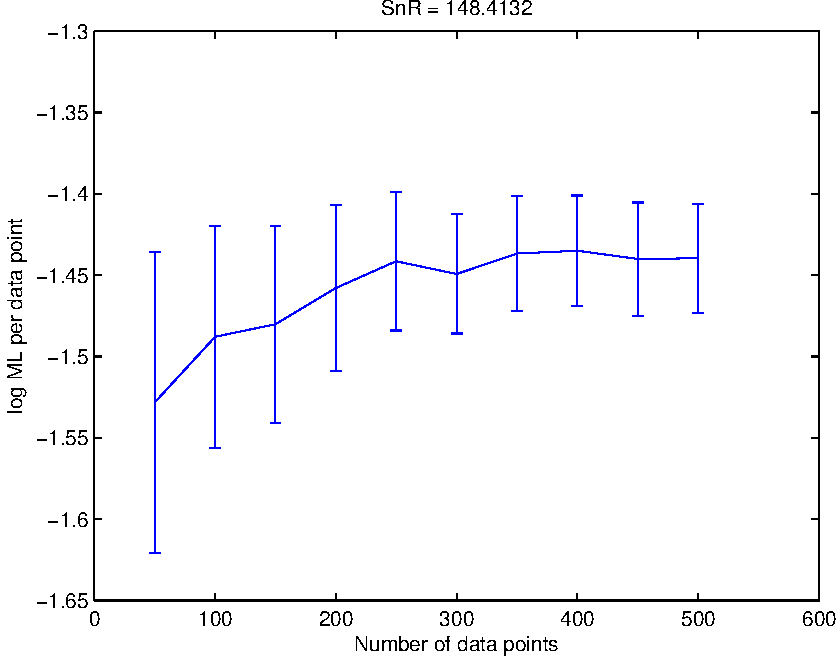
\includegraphics[width=0.32\columnwidth]{figures/ml-per-n/const}
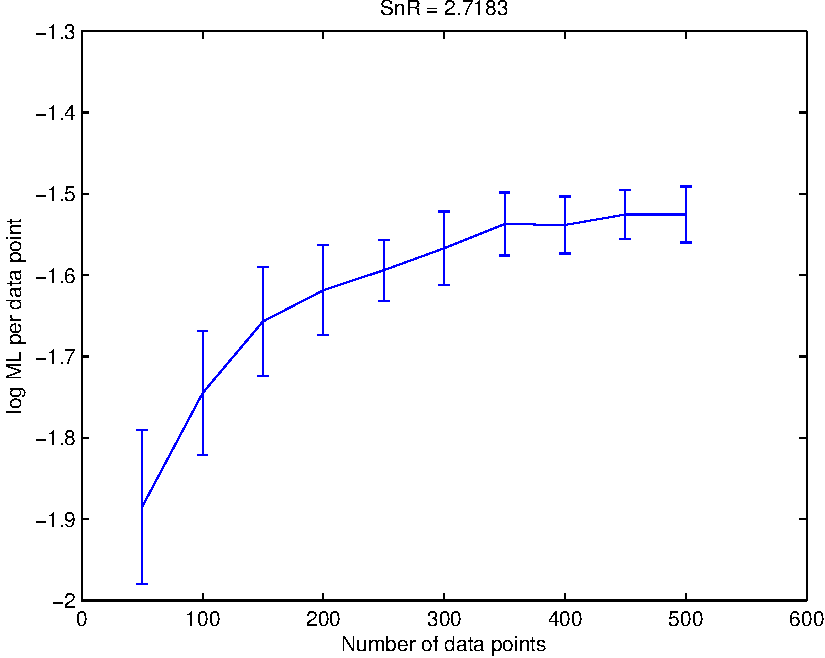
\includegraphics[width=0.32\columnwidth]{figures/ml-per-n/SE}
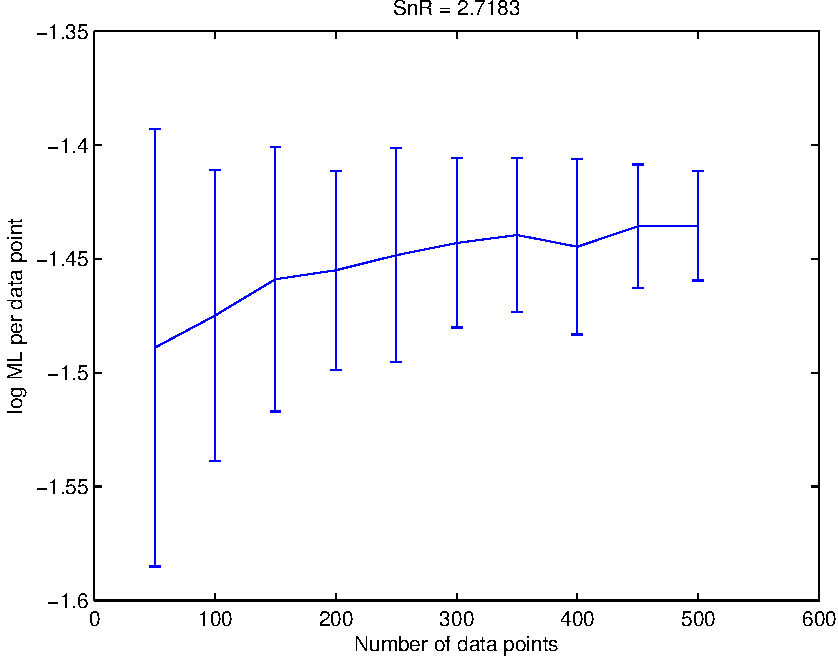
\includegraphics[width=0.32\columnwidth]{figures/ml-per-n/SE-longer}
\caption{
Left: Constant + noise.
Middle: Short lengthscale + noise.
Right: Longer lengthscale + noise.
}
\label{fig:lml_per_n}
\end{figure}

The figures show that the disagreement from proportionality decreases as the number of data points increases, but the amount of data required before this happens increases with the complexity / like of \iid-ness of the model.

For Bayes factors, the relative complexity of the models will determine if the equivalent of these plots tends to a constant from above or below.
So, something predicting changes in Bayes factors will have to estimate the current model complexity and the new model complexity as well as fit related terms which grow proportionally.

\subsection{Conclusions}

The scaling of marginal likelihoods depends on the model.
This scaling will depend on the models being compared and the true data generation process.
Doing fancy mathematics seems like a difficult route given that we ultimately need to predict the Bayes factor after running an optimiser.

\subsection{Next steps}

\begin{itemize}
  \item What statistics will best characterise the scaling of the marginal likelihood and Bayes factors?
  \item Or can we do some more mathematics?
\end{itemize}

\section{7 August - Some additional thoughts post AAAI}

Ultimately we may want to compare models for which marginal likelihoods are too complex to calculate.
We might instead use predictive likelihoods; possibily pointwise predictive likehoods (ignoring the joint distribution between all data points).
This would get round the Bayes factor scaling issue.

\subsection{Next steps}

\begin{itemize}
  \item Make a simple demonstration of this learning system working in 1d with SEs and PERs using Bayes factors and pointwise predictive likelihoods to demonstrate that the method is viable.
\end{itemize}

\newpage

%\appendix
%\section*{Appendix A.}
%Appendix

\vskip 0.2in
\bibliography{library}

\end{document}
